\chapter[LaTeX Docker]{LaTeX Docker\\\small{\textit{-- Charles, Justin, Benedict, Jacky}}}
\label{Chapter::LaTeX Docker}
\index{Chapter!LaTeX Docker}



\subsection{Project Directory Setup}
\begin{itemize}
    \item Create a folder docker-latex 
    \item Start docker
    \item Make sure docker is running by using docker run hello-world 
    \item cd into that folder directory 
\end{itemize}

\subsection{Docker Commands}
\begin{itemize}
    \item Create a Dockerfile with the content below
\end{itemize}

\begin{minted}{Bash}
FROM debian:bullseye-slim

ENV DEBIAN_FRONTEND=noninteractive

RUN apt-get update && \
    apt-get install -y \
        texlive-latex-base \
        texlive-latex-recommended \
        texlive-fonts-recommended \
        texlive-latex-extra \
        make \
        && apt-get clean && rm -rf /var/lib/apt/lists/*

WORKDIR /doc

CMD ["pdflatex", "main.tex"]
\end{minted}
\begin{itemize}
    \item Run nano main.tex and paste your desired LaTeX content 
    \item Build the docker image 
    \item Run the docker command 
    \item Check your folder to see if the main.pdf file is created 
\end{itemize}

\begin{minted}{Bash}
    nano main.tex
    docker build -t docker-latex . 
    docker run --rm -v "$PWD":/doc docker-latex
\end{minted}

\begin{figure}[htp]
    \centering
    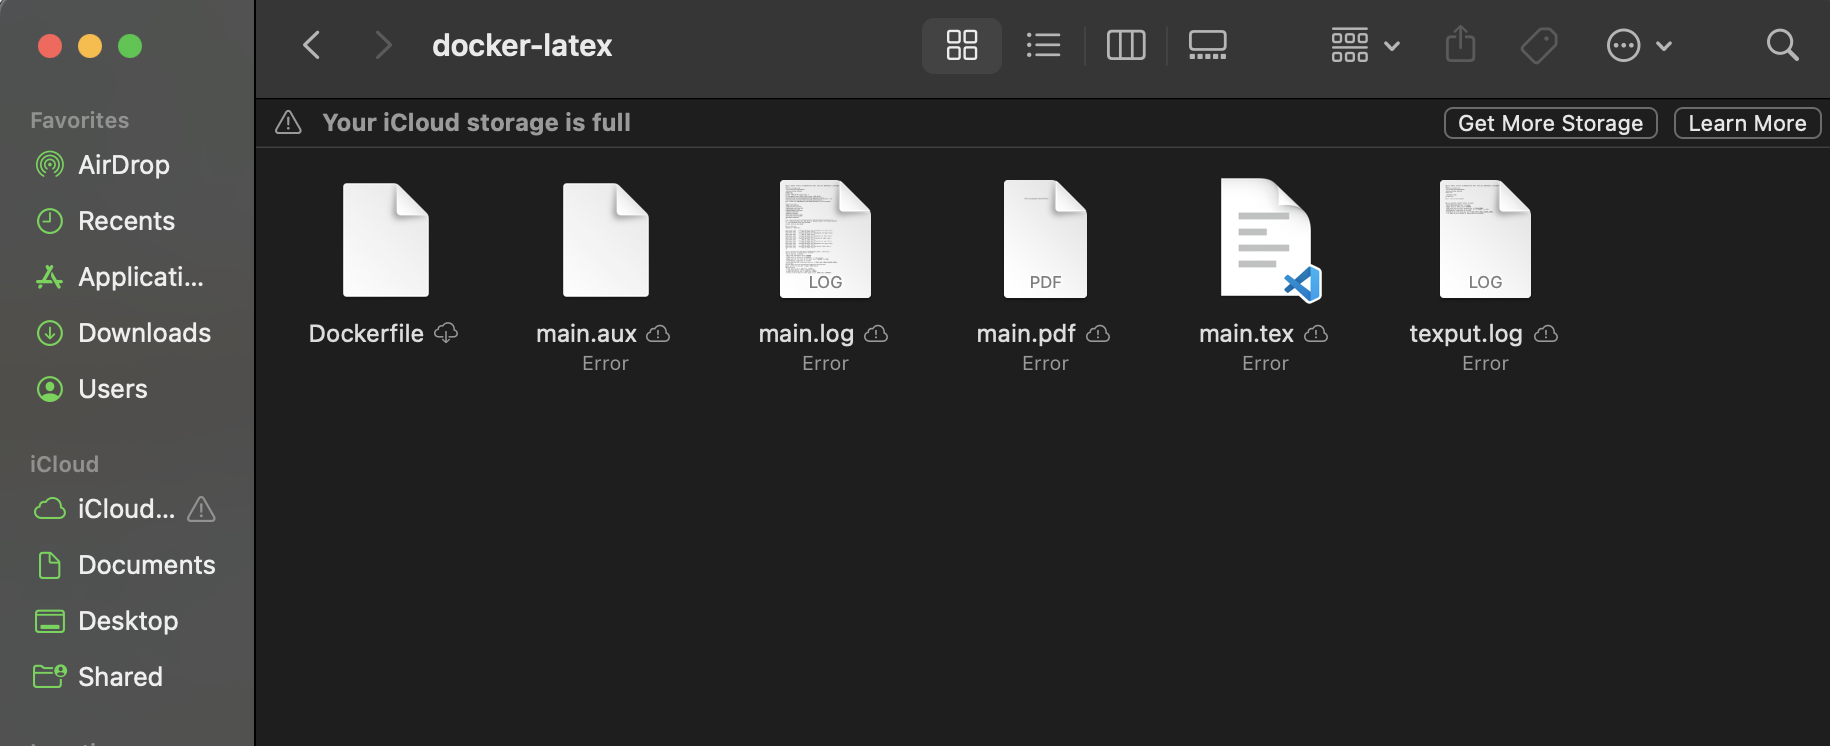
\includegraphics[width=15cm, height=10cm]{png/docker/docker-latex.png}
    \caption{Folder containing files created from successful Docker build}
    \label{fig:Part I Folder}
\end{figure}

\begin{figure}[htp]
    \centering
    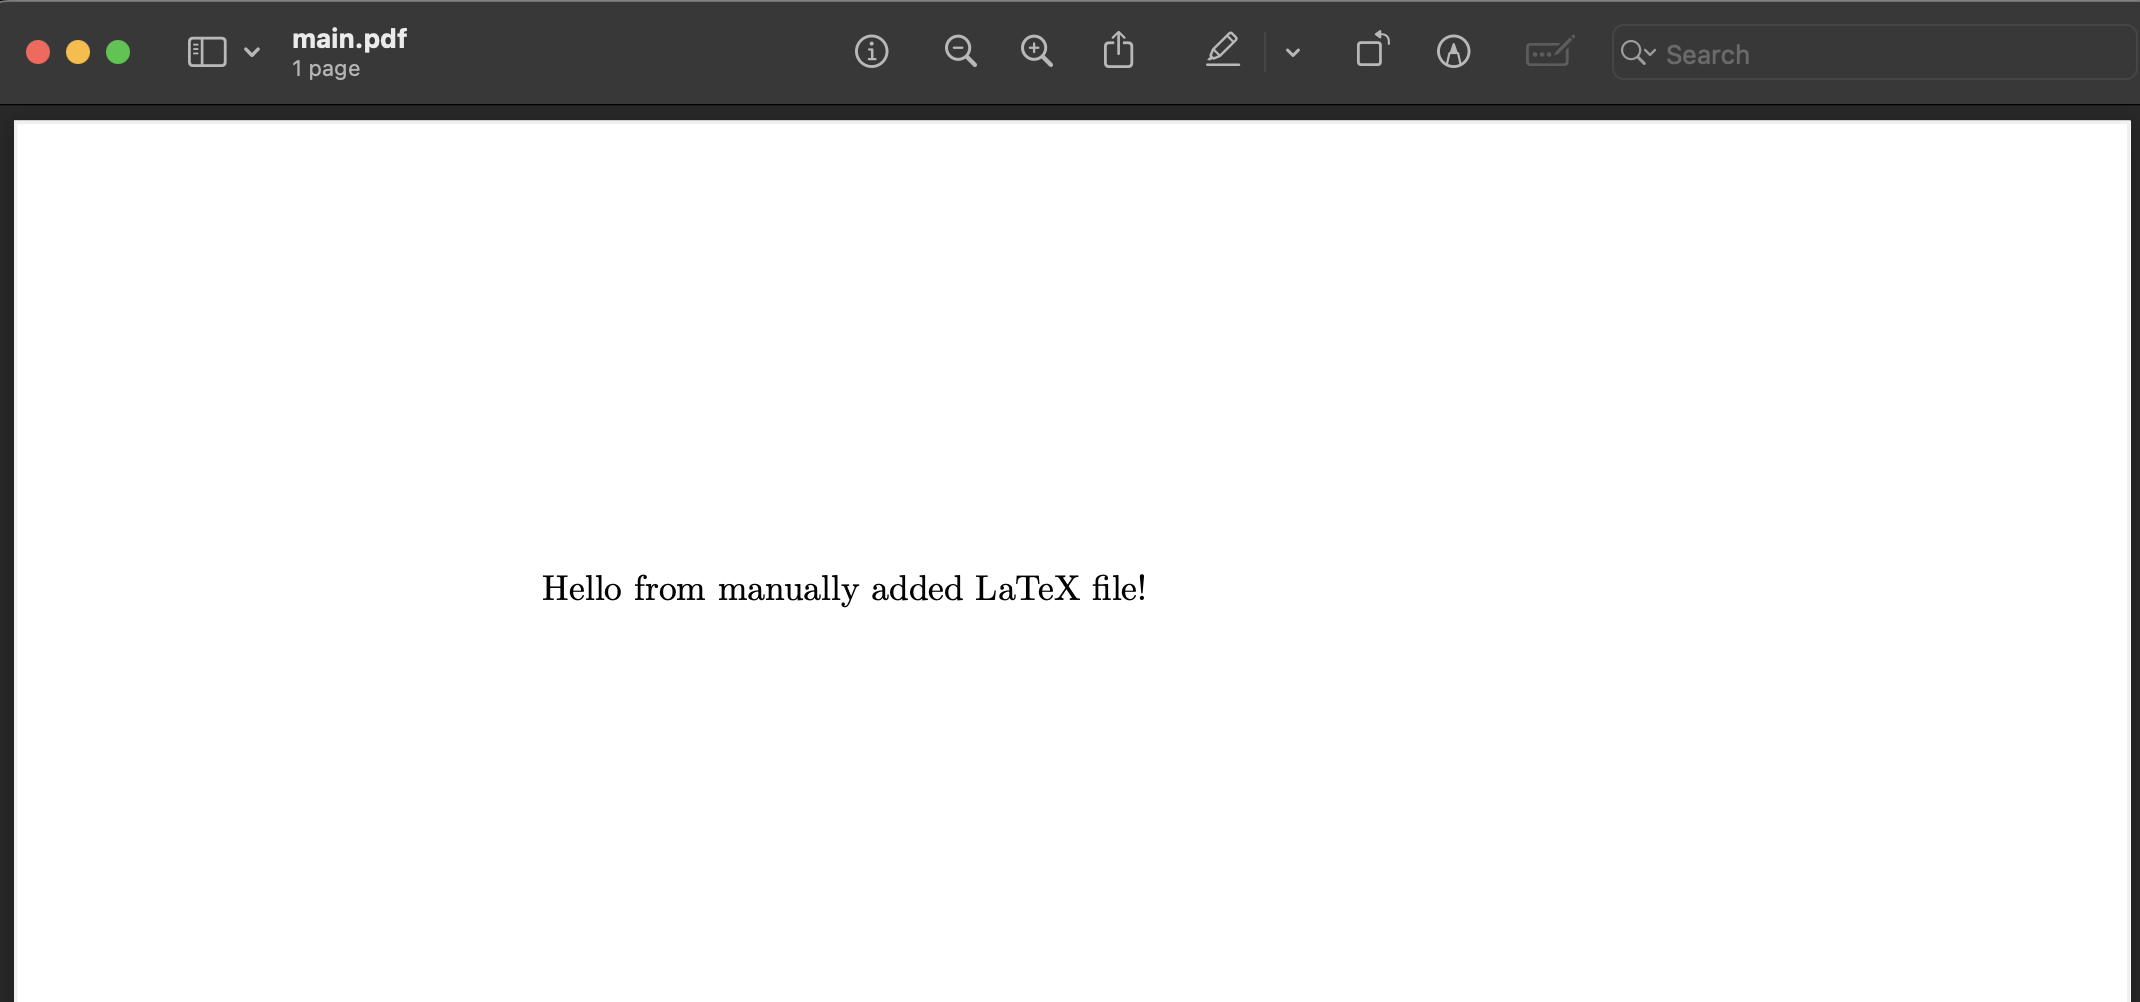
\includegraphics[width=15cm, height=10cm]{png/docker/docker_latex.png}
    \caption{Docker compiled LaTeX document}
    \label{fig:Part I LaTeX}
\end{figure}
